% !TEX root =  paper.tex
We propose an algorithm that unifies the UI component instances 
identified in the previous steps
into a component
implemented using a web framework (e.g., \react, \angular, \html Web Components~\cite{MDN:2017:WebComponents}).
However, instead of directly generating the framework-specific code for components,
we opt for constructing an \textit{intermediate model}
that effectively represents components at a higher level of abstraction.
This allows building different \textit{translation strategies}
for generating the actual code 
for different frameworks from the same model,
with the added benefit of remaining agnostic 
to the specific details of a particular framework. 
Our implementation supports the \react~\cite{React} translation strategy,
 which is the preferred framework for a significant number of developers in practice~\cite{StateOfJS:WebPlatformTests, StackOverflow:2017:Survey}.
We first define the terms used in this step.

\begin{defn}[\textbf{\mappedset}]
	\label{definition:mapped-nodes-set}
	Let $T = \{t_1 \ldots t_n\}$ be the list of \dom subtrees for $n$ instances
	of a UI component identified by the previous phases of the approach.
	%These subtrees are rooted at the \dom nodes located by the {\xpath}s 
	%returned by the previous phase.
    A set $D = \{d_1 \in t_1, d_2 \in t_2\ldots d_n \in t_n\}$ of \dom nodes corresponding to $T$
	is a \mappedset,
	when every pair $(d_i, d_j)$ of \dom nodes 
	belonging to $D$ are \textbf{mapping}.
\end{defn}

\begin{defn}[\textbf{Mapping}]
	Two \dom nodes $d_i$ and $d_j$
	are mapping (denoted as $d_i \leftrightsquigarrow d_j$) when:
	\begin{itemize}[leftmargin=*]
	\item Both $d_i$ and $d_j$ are root nodes of their trees, or 
	\item $d_i$ and $d_j$ are not root nodes, and
	\begin{itemize}[leftmargin=*]
		\item $d_i.parent.tag = d_j.parent.tag$, and
		\item $d_i.parent \leftrightsquigarrow d_j.parent$, and
		\item $d_i$ and $d_j$ have the same child index 
		(e.g., they are both the first child of their parents).
	\end{itemize}

	\end{itemize}
\end{defn}

\begin{defn}[\textbf{\model}]
	The \model is a rooted, ordered tree
	in which each node corresponds to a \mappedset.
	The hierarchy of this tree follows the mapping \dom nodes' hierarchy.
\end{defn}


\header{Example} \Cref{fig:intermediate-model-sample-dom-subtrees}(a) 
depicts the \html code snippets 
corresponding to two identified UI component instances.
%(the visual output is omitted due to space limitations).
The corresponding \dom subtrees,
and the constructed \model for these subtrees 
are respectively shown in \Cref{fig:intermediate-model-sample-dom-subtrees}(b) and (c).
The connected \dom nodes with dotted arrows form {\mappedset}s.
Notice that non-mapping \dom nodes do not form a node in the intermediate model.
This model can be translated to a \react-like component
similar to what is shown in \Cref{fig:intermediate-model-sample-dom-subtrees}(d).
Finally, the generated component is instantiated two times in the refactored \html code
to replace the originally-repeated \dom nodes.
The calls to the component can look like what is shown in \Cref{fig:intermediate-model-sample-dom-subtrees}(e).

\begin{figure}
    \centering
    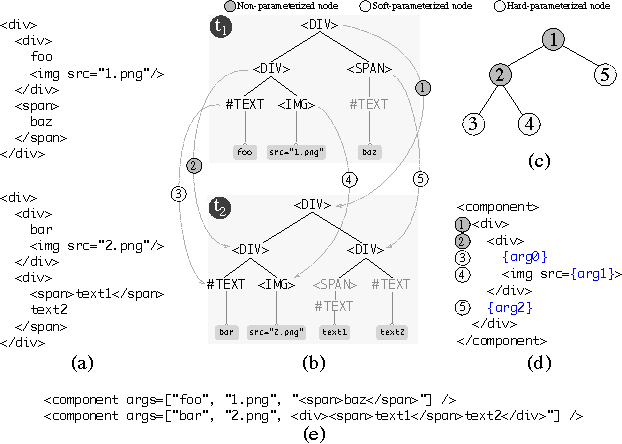
\includegraphics[width=0.70\textwidth]{maintainability/figures/intermediate-model}
    \caption{
    	(a) Initial \html code fragments.
     	(b) Corresponding \dom subtrees.
     	(c) The constructed \model.
     	(d) The final generated UI component.
     	(e) The \textit{calls} to the generated UI component.}
    \label{fig:intermediate-model-sample-dom-subtrees}
\end{figure} 

When generating the actual framework code,
each model node results into a \dom node in the framework component
(as depicted in \Cref{fig:intermediate-model-sample-dom-subtrees}(d)),
which essentially \textit{unify} the nodes in the \mappedset
to remove duplication.
There are three possibilities for framework component \dom nodes:

\begin{itemize}[leftmargin=*]

	\item When all pairs of \dom nodes in a \mappedset have the same tag and identical attribute values,
	they can be unified in one \dom node of the same tag.
	For example, the two \code{<div>} nodes in \Cref{fig:intermediate-model-sample-dom-subtrees}
	corresponding to model node \circled{1}
	form a \code{<div>} node in the component.
	
	\item A pair of \dom nodes in a \mappedset which have different tag names
	cannot be unified into one \dom node in the component
	(e.g., \code{<span>} and \code{<div>}
	corresponding to model node \circled{5} in \Cref{fig:intermediate-model-sample-dom-subtrees}).
	Similar is two text nodes with different content
	(e.g., the \code{foo} and \code{bar} corresponding to the model node \circled{3} in \Cref{fig:intermediate-model-sample-dom-subtrees}).
	In such cases, the \dom nodes (and the whole subtree rooted at them) should be \textit{hard-parameterized} in the resulting component,
	i.e., a \textit{placeholder} should be created.
	The original parameterized \dom nodes are later passed as \textit{arguments} when instantiating the component
	to recreate the original \dom hierarchy.
	
	\item A pair of \dom nodes in a \mappedset that have the same tag name but
	different values for one of their attributes
	might be unifiable into a \dom node 
	via \textit{soft parameterization},
	where the differing attribute values are parameterized
	(e.g., the \code{<img>} tags corresponding to model node \circled{4}
	in \Cref{fig:intermediate-model-sample-dom-subtrees},
	with parameterized \code{src} attribute values).
	This can be done only if the used framework supports parameterizing attribute values.
	Otherwise, the parameterization should be done as if it was a hard parameterization.

\end{itemize}

\header{The intermediate model construction and refactoring algorithm}
The inputs of \Cref{algorithm:refactoring} are the original mockup \html, 
the list of component instance \dom subtrees,
and the translation strategy.
The output is the refactored \html wherein duplication is removed using the UI components.

\begin{algorithm}
	\fontsize{7.5pt}{9pt}\selectfont
	%\linespread{1}\selectfont
	\caption{\model Generation}
	\label{algorithm:refactoring}
	% !TEX root =  paper.tex

\begin{algorithmic}[1]

\renewcommand{\algorithmicrequire}{\textbf{Input:}}
\renewcommand{\algorithmicensure}{\textbf{Output:}}

\Require \par ~ The original \dom of the mockup ($DOM_{original}$),
UI component instances \dom subtrees ($subtrees$), 
UI component translation strategy ($strategy$)

\Ensure The new \dom after refactoring ($DOM_{refactored}$)


\State $model \gets \Call{ConstructEmptyIntermediateModel}{{}}$ \label{algoline:ui-component-empty-model}
\State $coveredNodes \gets \varnothing$ \label{algoline:ui-component-covered-nodes-init}
\State $templateTree \gets \Call{getSmallestTree}{subtrees}$ \label{algoline:ui-component-template-tree}
\State $templateNodes \gets \Call{BFS}{templateTree}$
\For{$templateNode \in templateNodes \setminus coveredNodes$} \label{algoline:ui-component-main-loop-start}
	\State $coveredNodes \gets coveredNodes \cup \{ templateNode \}$
	\State $mappedNodes \gets \Call{getMappedNodesSet}{templateNode, subtrees}$\label{algoline:ui-component-mapped-nodes-set}
	\State $parameterization \gets \code{NULL}$
	\For{$currentNode \in mappedNodes \setminus coveredNodes $}
		\State $parameterization \gets \Call{compare}{templateNode,currentNode}$\label{algoline:ui-component-compare}
		\If{$parameterization \neq \code{NULL}$}
			\State \textbf{break} \label{algoline:ui-component-break}
		\EndIf
	\EndFor
	
	\State $parent \gets model.\Call{getModelNodeFor}{templateNode.parent}$\label{algoline:ui-component-add-model-nodes-start}
	
	\If{$parameterization \neq \code{NULL}$}
		\If{$parameterization = \code{SOFT\_PARAMETERIZATION}$ \par 
			\hspace{15mm} $\land strategy.\Call{supportsAttributeParameters}{{}}$}
			\State $model.\Call{addSoftParamNode}{parent, mappedNedesSet}$
			\State $coveredNodes \gets coveredNodes \cup mappedNodes$
		\Else
			\State $model.\Call{addHardParamNode}{parent, mappedNedesSet}$
			\State $coveredNodes \gets coveredNodes \cup $ \par 
				\hspace{20mm} $\Call{GetAllSubtreeNodes}{mappedNodes}$
		\EndIf
	\Else
		\State $model.\Call{addNonParamNode}{parent, mappedNedesSet}$
		\State $coveredNodes \gets coveredNodes \cup mappedNodes$
	\EndIf \label{algoline:ui-component-add-model-nodes-end}

\EndFor \label{algoline:ui-component-main-loop-end}
	

\State $DOM_{refactored} \gets strategy.\Call{refactor}{DOM_{original}, model}$ \label{algoline:ui-component-refactor}


\end{algorithmic}
\end{algorithm}

\Cref{algorithm:refactoring} starts by constructing an empty model (\cref{algoline:ui-component-empty-model}),
and an exclusion list (\code{coveredNodes} in \cref{algoline:ui-component-covered-nodes-init})
that contains the original \dom nodes of the component instances which are already covered by the algorithm
(e.g., a model node has been created for them),
so that they are skipped in future iterations.
To construct the intermediate model,
the algorithm chooses the \dom subtree of one of the component instances
(i.e., the \emph{template subtree}) to follow its hierarchy.
The template subtree is the one with the smallest number of \dom nodes,
chosen in \cref{algoline:ui-component-template-tree}.
This is because the intermediate model cannot have more  \dom nodes than the smallest subtree,
as it resembles the \textit{intersection} of the component instances' \dom subtrees.
The algorithm loops over all the uncovered template subtree's \dom nodes,
following the subtree's breadth-first traversal order
(lines~\ref{algoline:ui-component-main-loop-start} to \ref{algoline:ui-component-main-loop-end}).
Each template \dom node 
is compared to other \dom nodes of its \mappedset (identified according to \Cref{definition:mapped-nodes-set}
in \cref{algoline:ui-component-mapped-nodes-set})
using the \code{compare()} function (\cref{algoline:ui-component-compare}),
which returns the type of parameterization needed to unify two given \dom nodes,
and \code{NULL} if no parameterization is needed.
Note that, even if one node in a \mappedset should be parameterized 
when compared to the template \dom node, 
the resulting model node will be either hard- or soft-parameterized,
thus comparing other nodes of \mappedset is not required
(\cref{algoline:ui-component-break}).

The intuition behind comparing nodes in the breadth-first order is that,
across the component instances' \dom subtrees, it is more likely that the the inner nodes (which define the structure of the final UI component) 
are similar,
while the leaf nodes (texts, images) are more probable to differ.
%In addition, when a set of mapping inner nodes should be hard-parameterized,
%all the subtrees rooted at the mapping nodes should be parameterized,
%meaning that there will be no need to assess them in the future.
The inner nodes are thus compared before leaves,
also facilitating the identification of \mappedset based on \Cref{definition:mapped-nodes-set},
as the nodes' child indices follow the BFS traversal order. 
%\davood{I think DFS would be also possible}

The algorithm then continues to add a model node for each \mappedset
(lines~\ref{algoline:ui-component-add-model-nodes-start} to \ref{algoline:ui-component-add-model-nodes-end}).
First, the model node that has been created for the template \dom node's parent 
(in the previous runs of the loop) is retrieved from the model (\cref{algoline:ui-component-add-model-nodes-start}),
to which the new model nodes will be added as children.
This effectively allows the model to preserve the original hierarchy of the instances' \dom subtrees.
If the model is empty, the new model node will form the model's root.
The subsequent lines of the algorithm add the new model node
based on the parameterization type.
In each step, the \dom nodes in the \mappedset for which a model node is created
are added to the \code{coveredNodes} to be skipped in the next iterations.
As mentioned, in case of a hard-parameterized model node,
all the \dom nodes belonging to the subtrees rooted under the corresponding mapping \dom nodes
should be marked to be skipped (e.g., node \circled{5} in \Cref{fig:intermediate-model-sample-dom-subtrees}).

Finally, the actual refactoring is conducted using the constructed \model (\cref{algoline:ui-component-refactor}).
The details of the refactoring are built-in the translation strategy,
which can be implemented virtually for any UI framework of interest.



